\documentclass[12pt]{article}

\usepackage[portuguese]{babel}
\usepackage[utf8]{inputenc}
\usepackage{amsmath}
\usepackage{commath}
\usepackage[alf]{abntex2cite}
\usepackage{indentfirst}
\usepackage{graphicx}
\usepackage{multicol,lipsum}
\usepackage{geometry}
\usepackage[alf]{abntex2cite}
\usepackage{subfigure}
\graphicspath{{../../Figures/Report_19_09/}{../../Images/Report_19_09/}}

\geometry{
  paper = a4paper,
  inner = 3cm,
  outer = 3cm,
  top = 2cm,
  bottom = 2cm
}

\begin{document}
%\maketitle

\onehalfspacing

\begin{titlepage}
\begin{center}

\Huge{Universidade Federal de Alagoas}\\
\large{Instituto de Computação}\\ 
\large{Laboratório de Computação Científica e Análise Numérica}\\ 
\vspace{220pt}
\textbf{\LARGE{Research report}}\\
%\title{{\large{Título}}}
\vspace{3,5cm}
\end{center}

\begin{flushleft}
\begin{tabbing}
Student: Danilo Fernandes Costa\\
Professor: Alejandro Frery\\
\end{tabbing}
\end{flushleft}
\vspace{1cm}

\begin{center}
\vspace{\fill}
September\\
2019
\end{center}
\end{titlepage}

\section{Introduction}

In this report, some results of the analysis of samples referring to plantation regions observed over time are shown. The first observation was made on 16 May 2016, which was followed by four others with a time interval of 25 days between adjacent observations. 
Those regions consist of three soybeans crops, three wheat, two oats and two canola and are shown in the figures \ref{fig:r1} to \ref{fig:r5}. Those samples were obtained using the classification of the regions given in the figure \ref{fig:classes}.

\begin{figure}[hbt]
\centering
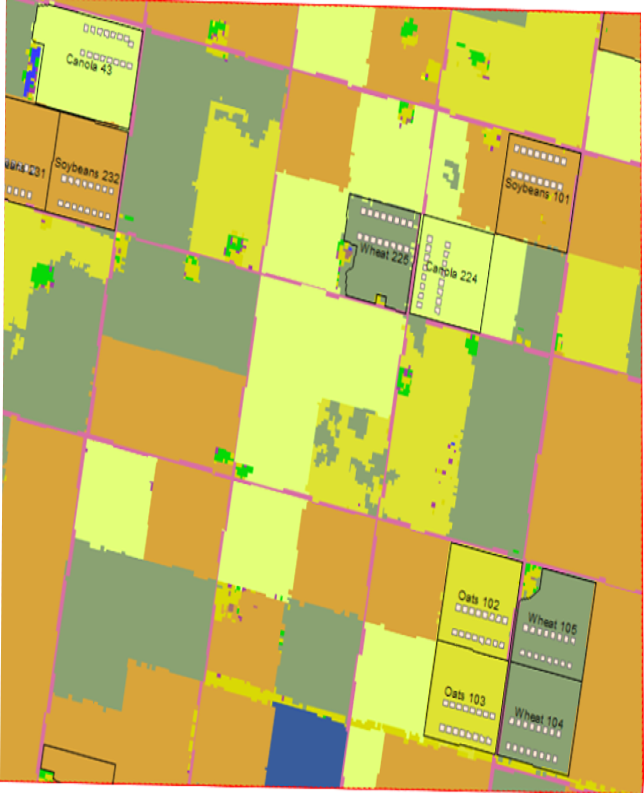
\includegraphics[width = .55\linewidth]{/Regions/classes}
\label{fig:classes}
\caption{Classification of the regions on the image}
\end{figure}

\begin{figure*}[hbt]
\centering

\subfigure[1th observation\label{fig:r1}]{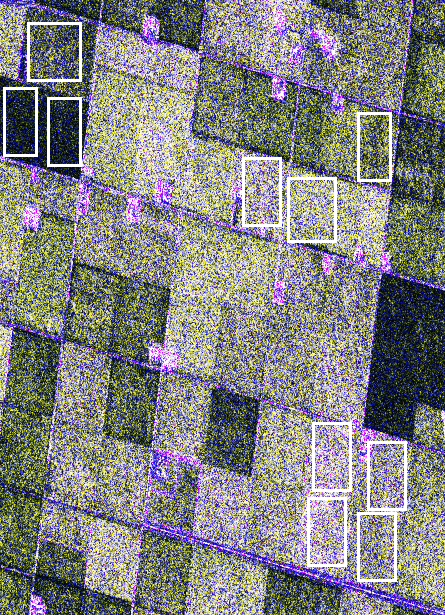
\includegraphics[width = .32\linewidth]{/Regions/regions_1}}
\subfigure[2th observation\label{fig:r2}]{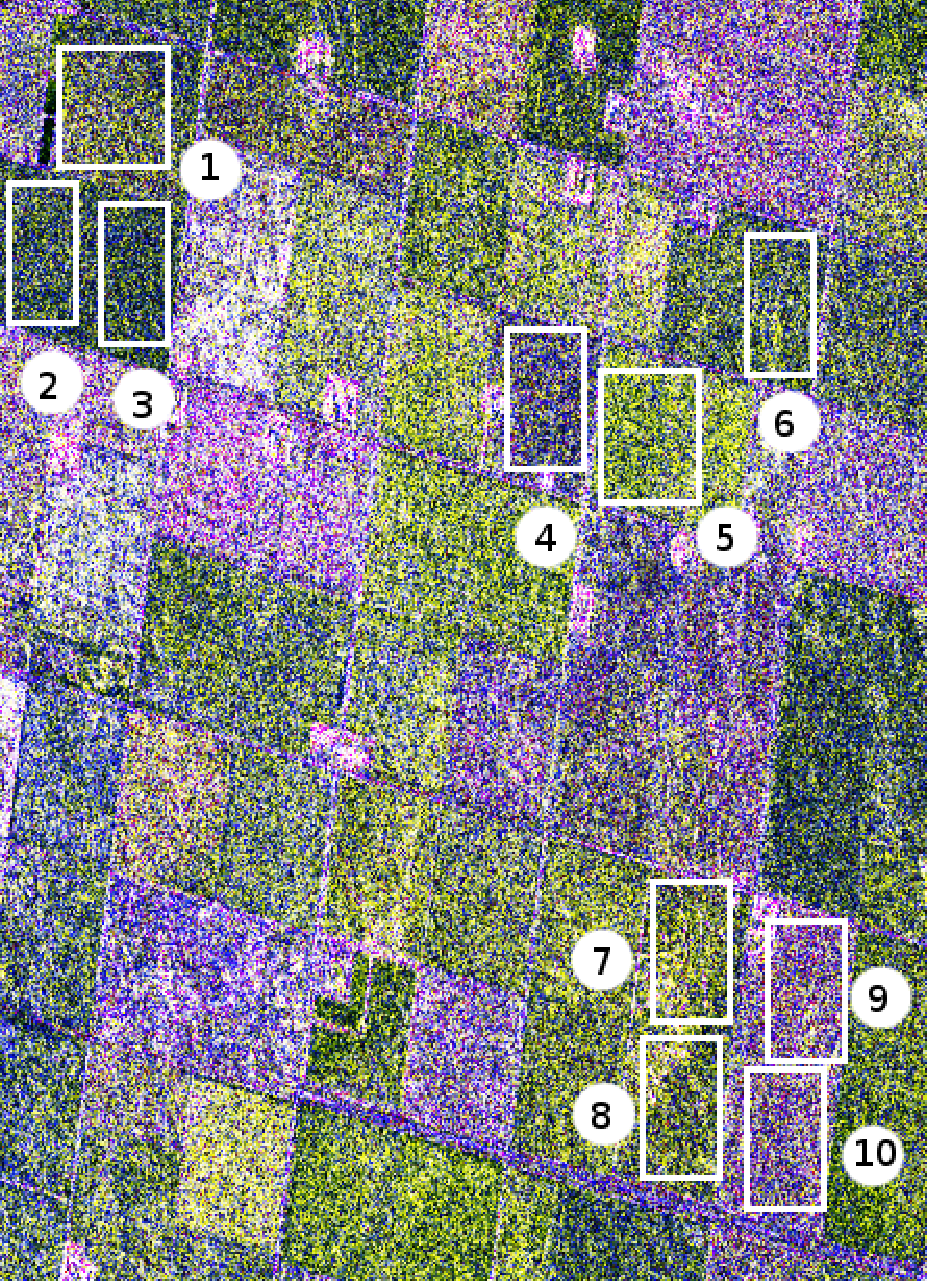
\includegraphics[width = .32\linewidth]{/Regions/regions_2}}
\subfigure[3th observation\label{fig:r3}]{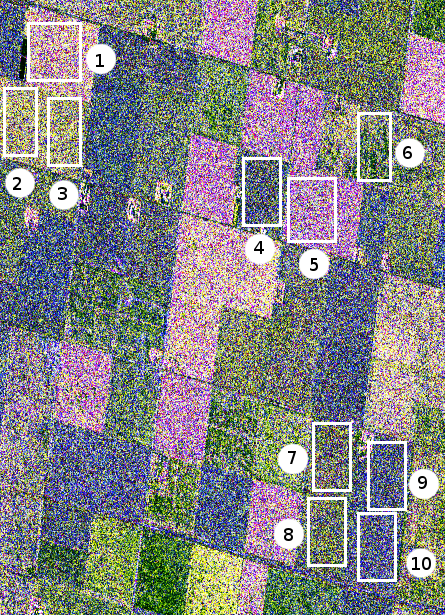
\includegraphics[width = .32\linewidth]{/Regions/regions_3}}
\subfigure[4th observation\label{fig:r4}]{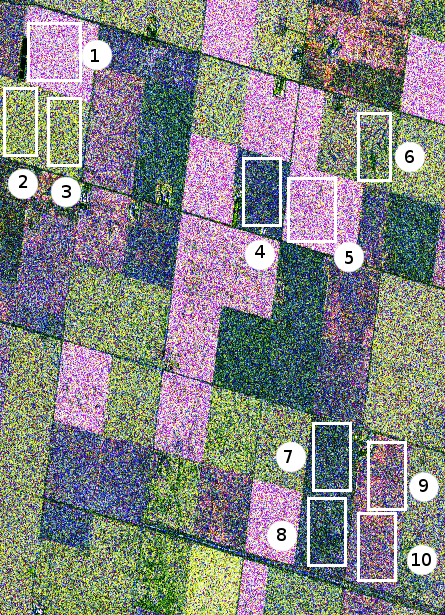
\includegraphics[width = .32\linewidth]{/Regions/regions_4}}
\subfigure[5th observation\label{fig:r5}]{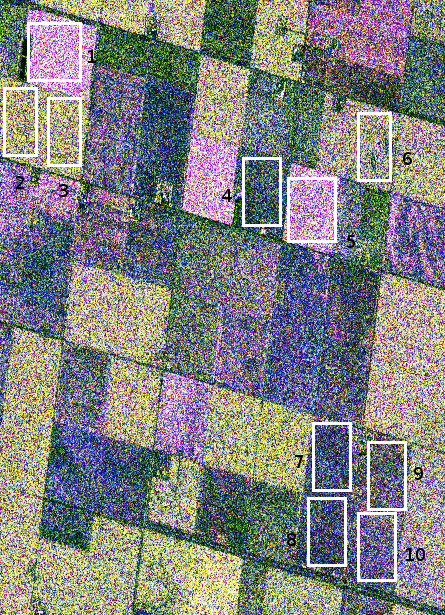
\includegraphics[width = .32\linewidth]{/Regions/regions_5}}

\caption{Samples analysed over time in where 1 to 10 corresponding respectively to Canola 43, Soybeans 231, Soybeans 232, Wheat 225, Canola 224, Soybeans 101, Oats 102, Oats 103, Wheat 105 and Wheat 104}
\label{fig:regions}
\end{figure*}

\end{document}